%%%%%%%%%%%%%%%%%%%%%%%%%%%%%%%%%%%%%%%%%%%%%%%%%%%%%%%%%%%%%%%%%%%%%%%%%%%%
% AGUtmpl.tex: this template file is for articles formatted with LaTeX2e,
% Modified April 2011
%
% This template includes commands and instructions
% given in the order necessary to produce a final output that will
% satisfy AGU requirements.
%
% PLEASE DO NOT USE YOUR OWN MACROS
% DO NOT USE \newcommand, \defcommand, or \renewcommand. 
%
%
%%%%%%%%%%%%%%%%%%%%%%%%%%%%%%%%%%%%%%%%%%%%%%%%%%%%%%%%%%%%%%%%%%%%%%%%%%%%
%
% All questions should be e-mailed to latex@agu.org.
%
%%%%%%%%%%%%%%%%%%%%%%%%%%%%%%%%%%%%%%%%%%%%%%%%%%%%%%%%%%%%%%%%%%%%%%%%%%%%
%
% Step 1: Set the \documentclass
%
% There are two options for article format: two column (default)
% and draft.
%
% PLEASE USE THE DRAFT OPTION TO SUBMIT YOUR PAPERS.
% The draft option produces double spaced output.
%
% Choose the journal abbreviation for the journal you are
% submitting to:

% jgrga JOURNAL OF GEOPHYSICAL RESEARCH
% gbc   GLOBAL BIOCHEMICAL CYCLES
% grl   GEOPHYSICAL RESEARCH LETTERS
% pal   PALEOCEANOGRAPHY
% ras   RADIO SCIENCE
% rog   REVIEWS OF GEOPHYSICS
% tec   TECTONICS
% wrr   WATER RESOURCES RESEARCH
% gc    GEOCHEMISTRY, GEOPHYSICS, GEOSYSTEMS

% (If you are submitting to a journal other than jgrga,
% substitute the initials of the journal for "jgrga" below)

%\documentclass[draft,grl]{AGUTeX}  % @@@@@@@@@@@@@@@@@

%%%%%%%%%%%%%%%%%%%%%%%%%%%%%%%%%%%%%%%%%%%%%%%%%%%%%%%%%%%%%%%%%%%%%%%%%
% OPTIONAL:
% To produce a two-columned version:
\documentclass[grl]{AGUTeX}  % @@@@@@@@@@@@@@@@@@

% Two-columned format can be used to estimate the number of pages
% for the final published PDF.

% PLEASE USE THE DRAFT OPTION TO SUBMIT YOUR PAPERS.
%%%%%%%%%%%%%%%%%%%%%%%%%%%%%%%%%%%%%%%%%%%%%%%%%%%%%%%%%%%%%%%%%%%%%%%%%
% OPTIONAL:
% To create numbered lines:

% If you don't already have lineno.sty, you can download it from
% http://www.ctan.org/tex-archive/macros/latex/contrib/ednotes/
% (or search the internet for lineno.sty ctan), available at TeX Archive Network (CTAN).
% Take care that you always use the latest version.

% To activate the commands, uncomment \usepackage{lineno}
% and \linenumbers*[1]command, below:

%\usepackage{lineno} % @@ use with drafts
%\linenumbers*[1]       % @@ use with drafts

%  To add line numbers to lines with equations:

%  \begin{linenomath*}
%  \begin{equation}
%  \end{equation}
%  \end{linenomath*}
%%%%%%%%%%%%%%%%%%%%%%%%%%%%%%%%%%%%%%%%%%%%%%%%%%%%%%%%%%%%%%%%%%%%%%%%%
% Figures and Tables
%
% When submitting articles through the GEMS system:
% COMMENT OUT ANY COMMANDS THAT INCLUDE GRAPHICS.
% (See FIGURES section near the end of the file.)

%  Figures and tables should be placed AT THE END OF THE ARTICLE,
%  after the references.
%
%  Uncomment the following command to include .eps files
%  (comment out this line for draft format):
%@@ \usepackage[dvips]{graphicx}
 
\usepackage{graphicx}
\usepackage{color}
\usepackage{lscape}

%
%  Uncomment the following command to allow illustrations to print
%   when using Draft:
  \setkeys{Gin}{draft=false}  % @@
%
% Substitute one of the following for [dvips] above
% if you are using a different driver program and want to
% proof your illustrations on your machine:
%
% [xdvi], [dvipdf], [dvipsone], [dviwindo], [emtex], [dviwin],
% [pctexps],  [pctexwin],  [pctexhp],  [pctex32], [truetex], [tcidvi],
% [oztex], [textures]
%
% See how to enter figures and tables at the end of the article, after
% references.
%
%% ------------------------------------------------------------------------ %%
%
%  ENTER PREAMBLE
%
%% ------------------------------------------------------------------------ %%

% Author names in capital letters:
\authorrunninghead{MCCUSKER ET AL.}

% Shorter version of title entered in capital letters:
\titlerunninghead{SHORT TITLE}

% Author mailing address: please repeat this command for
% each author and alphabetize authors:

%\authoraddr{D. S. Battisti,
%Department of Atmospheric Sciences, University of
%Washington, Seattle, WA 98135, USA. }
%
%\authoraddr{C. M. Bitz,
%Department of Atmospheric Sciences, University of
%Washington, Seattle, WA 98135, USA. }

\authoraddr{J. C. Fyfe,
Canadian Centre for Climate Modelling and Analysis, 
Victoria, BC V8V 1B5, Canada.}

\authoraddr{K. E. McCusker,
School of Earth and Ocean Sciences, University of
Victoria, Victoria, BC V8V 1B5, Canada.
(kemccusk@uvic.ca)}

\authoraddr{M. Sigmond,
Canadian Centre for Climate Modelling and Analysis, 
Victoria, BC V8V 1B5, Canada.}

%\authoraddr{R. C. Bales,
%Department of Hydrology and Water Resources, University of
%Arizona, Harshbarger Building 11, Tucson, AZ 85721, USA.
%(roger@hwr.arizona.edu)}

%\authoraddr{J. R. McConnell, Division of Hydrologic
%Sciences, 123 Main Street, Desert Research Institute, Reno, NV
%89512, USA.}

%\authoraddr{E. Mosley-Thompson, Department of Geography,
%Ohio State University, 123 Orange Boulevard, Columbus, OH 43210,
%USA.}

%\authoraddr{R. Williams, Department of Space Sciences, University of
%Michigan, 123 Brown Avenue, Ann Arbor, MI 48109, USA.}

%\authoraddr{Francesco Visconti, Dipartimento di Idraulica, 
%Trasporti ed Infrastrutture Civili, Politecnico di Torino, 
%Corso Duca degli Abruzzi 24, I-10129, Torino, Italy.

\begin{document}

%% ------------------------------------------------------------------------ %%
%
%  TITLE
%
%% ------------------------------------------------------------------------ %%

%\title{No link between human-induced Arctic sea ice loss and cold Eurasian winters}
\title{Tenuous link between human-induced Arctic sea ice loss and cold Eurasian winters}

% e.g., \title{Terrestrial ring current:
% Origin, formation, and decay $\alpha\beta\Gamma\Delta$}
%

%% ------------------------------------------------------------------------ %%
%
%  AUTHORS AND AFFILIATIONS
%
%% ------------------------------------------------------------------------ %%


%Use \author{\altaffilmark{}} and \altaffiltext{}

% \altaffilmark will produce footnote;
% matching \altaffiltext will appear at bottom of page.

\authors{K. E. McCusker,\altaffilmark{1}, J. C. Fyfe,\altaffilmark{2}, M. Sigmond,\altaffilmark{2}}

\altaffiltext{1}{School of Earth and Ocean Sciences,
University of Victoria, Victoria, British Columbia, Canada.}
\altaffiltext{2}{Canadian Centre for Climate Modelling and Analysis,
Victoria, BC, Canada.}

% ----- figure options from wikibook
% h	Place the float here, i.e., approximately at the same point it occurs in the source text (however, not exactly at the spot)
% t	Position at the top of the page.
% b	Position at the bottom of the page.
% p	Put on a special page for floats only.
% !	Override internal parameters LaTeX uses for determining "good" float positions.
% H	Places the float at precisely the location in the LaTeX code. Requires the float package,[1] e.g., \usepackage{float}. This is somewhat equivalent to h!.
% ---------
% @@@@@@ can have 3,000 words, plus 6 figures or 3500 + 5 figures (12 publishing units)
%    units: 500words =  figure = table = 1 unit.  12 maximum units.  % @@@@@

%% ------------------------------------------------------------------------ %%
%
%  ABSTRACT
%
%% ------------------------------------------------------------------------ %%

% >> Do NOT include any \begin...\end commands within
% >> the body of the abstract.

\begin{abstract}
Observed Arctic sea ice loss has been implicated in the recent prevalence of anomalously cold winters in Eurasia. Whether this linkage is a robust feature of anthropogenic sea ice loss, however, remains an open question because observed sea ice loss is due to a combination of external (human-induced) forcing and internal (random) variability. The interpretation of any warm Arctic-cold Eurasia linkages is further complicated by large wintertime internal variability over midlatitude land in observations and in atmospheric model simulations that attempt to isolate the response to sea ice loss. Here we execute two large ensembles ($>$600 years per ensemble) of simulations in an atmospheric general circulation model with prescribed historical sea ice loss taken from five historical simulations in the associated coupled global climate model in order to isolate the impact of past human-induced sea ice loss, as distinct from observed sea ice loss, on Eurasian temperature. We find the average Eurasian temperature response is negligible due to human-induced sea ice loss, however we find long periods (120 years) of both significant warming and cooling over Eurasia in early winter, linked to geopotential height anomalies over the Barents-Kara Seas region of the Arctic. This suggests that observed cold winters are largely due to internal variability in the sea ice itself combined with internal variability in the response to human-induced sea ice loss.
\end{abstract} % if need to add citations: First sentence: Kim, Mori, P&M13, Overland11, Liu12, Inoue12,P&S10. Sentence 3: ScreenClimDyn13
%% ------------------------------------------------------------------------ %%
%
%  BEGIN ARTICLE
%
%% ------------------------------------------------------------------------ %%

% The body of the article must start with a \begin{article} command
%
% \end{article} must follow the references section, before the figures
%  and tables.

\begin{article}

%% ------------------------------------------------------------------------ %%
%
%  TEXT
%
%% ------------------------------------------------------------------------ %%


%\section{Introduction}

Internal variability in the climate system plays an important role in determining the evolution of Arctic sea-ice extent (cite Wettstein14, Swart15), contributing approximately 50\% to the magnitude of the observed trend (cite Stroeve07, Kay11). Recent reductions in Arctic sea-ice area (cite@@) have coincided with an apparent prevalence of colder wintertime surface air temperature over Eurasian land surfaces (cite@@), prompting associations to be drawn in the literature between the two observed phenomena (cite Francis12,Mori14, Kim14, Inoue12, Overland11, Liu12,Petoukhov10,Honda09,Peings13). The frequency of anomalously cold Eurasian surface air temperatures (SAT) in winter is particularly sensitive to observed sea-ice loss in the Barents-Kara Seas region through Rossby wave propogation incited by increased surface heat fluxes (Peings13,Kim14,Mori14,Honda09). %(@@need to say more about uncertainties in previous work@@)  cite Screen13 re: significance. What is new here is that we DO get significance that is in the end, not robust, which is different than Screen's points.

Distinguishing a robust Arctic sea ice -- Eurasian SAT linkage is complicated by the large internal variability in atmospheric circulation and SAT in the mid-latitudes (cite Deser12). Indeed, Honda et al. (2009), who find that BKS sea-ice loss causes late-winter Eurasian cooling in an AGCM, state that their results are significantly weakened if all integrations are included in their averaging instead of a subset. Furthermore, much of the 'forcing' in these scenarios, the observed sea ice change, is itself also due to internal variability. Thus, a critical question remains: Has human-induced sea ice loss caused colder Eurasian winter temperatures? Answering this is important because unlike intrinsic variability that is by definition chaotic, the anthropogenic signal is theoretically identifiable and meaningful for future implications, as the anthropogenic signal will continue to grow and potentially emerge from the noise of internal variability.

%Our aim is to isolate the effect of human-induced sea-ice loss on the atmosphere because i. the anthropogenic signal is theoretically identifiable and robust whereas internal variability is by definition chaotic, and ii. the anthropogenic signal will likely continue to grow, potentially emerging from the noise of internal variability. 
%The answer to this has more-direct implications for future sea-ice loss. 
%Given that internal variability in surface air temperature (SAT) in the mid-latitudes is very large (cite Deser12) and much of the sea ice change itself is also due to internal variability, linkages drawn from observations are not able to illuminate the influence that human-induced sea-ice loss has on Eurasian SAT. % limited in their ability to provide knowledge about how human-induced sea-ice loss has influenced Eurasian SAT. %do not tell us anything about the influence that human-induced sea-ice loss has on Eurasian SAT.
%Sea ice loss in the Barents and Kara Seas region (BKS) has been pointed to as a primary driver of anomalously cold Eurasian surface air tempuratures (SAT) through Rossby wave propagation incited by increased surface heat fluxes (Peings13,Kim14,Mori14,Honda09).
% While associations do not imply causation, Physical mechanisms   .. well-supported by modelling ...

% Results
A clear anthropogenic signal in Arctic sea ice area changes in early winter (Nov-Dec; ND) since 1979 is already evident, demonstrated by the separation of histograms in Figure 1. The histograms show ND sea ice area changes from 1979-89 to 2002-12 from 50 simulations executed in the Canadian Earth System Model v2 (CanESM2) that are forced with all historical forcings (Historical; red), and 50 simulations forced with only natural forcings (HistoricalNat; gray. See Methods). Whereas natural forcing yields nearly equal chances of sea-ice growth and sea-ice loss, including anthropogenic forcing always yields sea-ice loss even with the large spread from internal variability. Estimates of sea ice loss from satellite measurements over the same time period are shown as green (National Sea Ice Data Center; NSIDC) and blue (Hadley Centre sea ice and SST dataset v1.1; HadISST) circles on the Historical curve fit. Observations represent one potential reality out of many, and thus are not expected to fall in any particular place on the Historical distribution. The CanESM2 Historical ensemble compares favourably with the NSIDC observations, however we note that the HadISST data, which are known to have biases in shoulder seasons@@, underestimate sea-ice loss and fall within the HistoricalNat distribution. %This may have implications for previous work utilizing the HadISST dataset to study the Arctic sea ice -- Eurasian SAT connection. %  demonstrates the clear signal of anthropogenic forcing in Arctic sea ice area since 1979, as well as the large influence of internal variability in determining these changes. 

Here we show the powerful and sometimes misleading effect internal variability can have on the response of Eurasian SAT to Arctic sea ice loss using two large ensembles of atmospheric general circulation model (AGCM) simulations. Pairs of simulations are executed with the associated Canadian AGCM in which past (1979-89) and present-day (2002-12) Arctic sea-ice conditions from the five CanESM2 Historical ensemble members that are included as part of CMIP5 (anomalies shown as red circles in Figure 1) are prescribed as boundary conditions (Methods). Annually-repeating, monthly sea-ice concentration (SIC), sea-ice thickness (SIT), and local sea surface temperature (where SIC $<$ 15\% in the present day but not the past) are prescribed and executed for 120 years each for 'past' conditions and 'present-day' conditions for each of five boundary conditions ('Individual SIC forcing' ensemble). We similarly execute five pairs of 120-year simulations, differing only in their initial conditions, with the average of the five Historical ensemble members as boundary conditions ('Average SIC forcing' ensemble) to represent the 'human-induced' forcing in which internal variability is averaged out. Thus in total, each ensemble consists of 600 years of (present - past) anomalies.

Figure 2a shows early winter polar SAT changes in the Individual SIC forcing ensemble (black) and in the Average SIC forcing ensemble (red) as 'uncertainty cascades' (cite Wilby10?) to illustrate the effect of variable boundary conditions versus internal variability in the response to sea-ice loss. The average of all five sets of 120-year anomalies (or 'superensemble average') is shown as the top level of each cascade, with individual 120-year averages making up the middle, and two subsampled 60-year averages for each 120-year member constituting the bottom. While the superensemble average polar SAT responses are similar and not statistically different from one another, the effect of variable boundary forcing in the top cascade is apparent in the larger range of 120-year polar SAT responses, despite the fact that the variance in the 120-year averages is not statistically different at the 95\% level (it is significantly different in Sep-Oct averages; not shown). In all cases, the polar SAT over present-day Arctic SIC is significantly different from the SAT over past SIC at the 95\% level, as indicated by the filled circles (Methods). %We can learn two things from this, the first being that the polar SAT response is additive, in that the response to the mean forcing is the same as the mean response to the individual forcings. @@is the variance statistically diff at the 90% level? think so?..@@ %The superensemble averages of polar SAT are not statistically different from each other at just under 1.8$^\circ$C, however what makes up the averages varies based on the boundary forcing;  %the effect of variable sea-ice boundary conditions is evident when comparing the range of polar SAT in the individual 120-year averages in level two between the two ensembles. The magnitude of polar SAT response in Nov-Dec is directly tied to the magnitude of sea ice loss and can be explained by the maximum in surface heat flux that occurs in these months@@

The SAT response over Eurasia (35$^\circ$N-60$^\circ$N, 40$^\circ$E-120$^\circ$E), however, is not statistically different from zero in both superensemble averages (Fig. 2b), indicating that the robust response of Eurasian temperature to Arctic sea-ice loss is essentially no response. Nevertheless, two of the 'Individual SIC forcing' ensemble members do have statistically significant Eurasian SAT anomalies at the 95\% level --- one a cooling of about -0.3$^\circ$C, and one a warming of about 0.3$^\circ$C. Moreover, the 'Average SIC forcing' ensemble members with the maximum and minimum anomalies are nearly significant at the 95\% level, and are significant at 90\%. Even a few 60-year average anomalies are also significant. In Eurasian SAT, and certainly circulation variables (not shown), the effect of differing boundary forcing is overpowered by the internal variability in the response. This is illustrated by the comparable uncertainty in the 120-year average anomalies between the two ensembles.  %Each of these SAT responses, spatially averaged over Eurasia, are statistically significant at the 95\% level using the Student's T test difference of means between the 120-years of the 'past' sea-ice simulation and the 120-years of the 'present-day' sea-ice simulation.

We have seen that Arctic sea-ice loss can yield both warmer and cooler Eurasian SATs in early winter, even with a large ensemble size of 120-years each (top of Fig. 2b). Unexpectedly, identical sea-ice boundary forcing also yields Eurasian SAT responses of opposing signs (bottom of Fig. 2b). To understand this further, we show in Figure 3 the spatial maps of SAT (shading) and geopotential heights at 500 mb (Z500; contours) over Eurasia for the two extreme cases in the 'Individual SIC forcings' ensemble. The circulation response associated with these SAT patterns are quite different from one another and in some locations, nearly opposite. The cooling case (Fig. 3a) shows an increase in Z500 to the north and a weak decrease over central Eurasia. This pattern is conducive for advection of polar air to the south and west along Z500 contours, and is particularly favourable in the region just over and south of the Barents-Kara Seas, just visible in the north-northcenter of the image. In contrast, the warming case (Fig. 3b) exhibits a decrease in Z500 in that same region, with increases over the southern continent and the northeast. This pattern favours warm-moist air advection from the south and west. % @@also say something about the SLP pattern which is more directly associated w/ changes in SIC  %, and is similar to @@prev studies? Neg AO?@@ Meanwhile, the warming case     % look at these two cases and their z500 responses over polar cap and bks only -- are they significant? prob no..@@@

The relationship between early winter circulation over the Barents-Kara Seas and Eurasian SAT is genuine and is displayed across 120-year ensemble member averages in Figure 4. As the 120-year average Z500 anomalies over the Barents-Kara Seas increase, 120-year average Eurasian SAT decreases, with a regression slope of @@, and a p-value of 0.054. This same relationship also holds within each individual simulation in time (not shown). Thus, the physical mechanisms that lead to the Eurasian cooling case are consistent with existing work that points to the Barents-Kara Seas region, however the fundamental origin is not sea-ice concentration changes (or SST changes as suggested by Sato13) as evidenced by the existence of a range of Z500/Eurasian SAT responses for identical SIC and SST in the Barents-Kara Seas (red circles in Fig. 4). %@@@@ look at fluxes in BKS  %However, not all positive Z500 anomalies produce negative SAT anomalies. 






% The histograms of November-December averaged sea ice area anomalies between 2002-12 and 1979-89 from two large ensembles executed with the Canadian Earth System Model version 2 (CanESM2) shown in Figure 1 highlight the clear signal of anthropogenic forcing (separation of Historical and HistoricalNat distributions) as well as the role of internal variability (spread of each distribution). 

%Figure 1, which shows histograms of November-December averaged sea ice area anomalies between 2002-12 and 1979-89 from two large ensembles executed with the Canadian Earth System Model version 2 (CanESM2), shows t the clear signal of anthropogenic sea ice-

%We do this by executing two large ensembles of paired simulations (1979-89 average boundary conditions and 2001-12 average boundary conditions) with prescribed Arctic sea ice concentration (SIC) and sea surface temperature (SST) boundary conditions. One ensemble ('Variable SIC forcings') is made up of five 


%\section{Methods}



%\section{Results}



\begin{figure}[t] %[h!]
  \noindent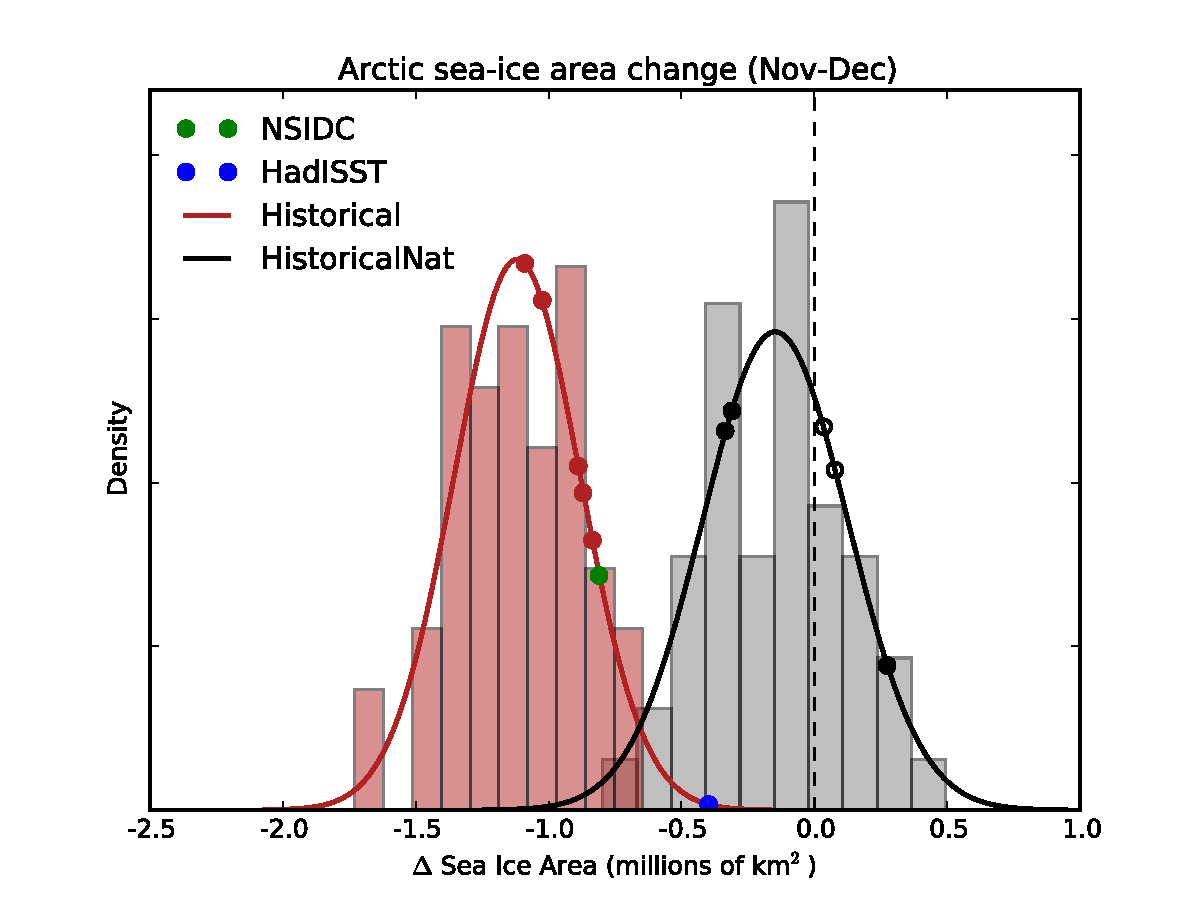
\includegraphics[width=20pc,angle=0]{fig1.pdf} \\ 
  \caption{Histograms and histogram fits of November-December averaged Arctic sea-ice area changes from the period 1979-89 to 2002-12 in the CanESM Historical (red) and HistoricalNat (gray) large ensembles (50 members each). Red markers indicate the original five Historical simulations, published as part of CMIP5 and seeds for the Historical LE, and also prescribed as boundary conditions to our 'Individual SIC forcings' AGCM simulations. Black markers are as red except for the HistoricalNat simulations. Green and blue markers show Arctic sea-ice change from two observational datasets. Filled markers indicate the present day period (2002-12) is significantly different from the past (1979-89) at the 95\% level using the Student's T test of difference between two means.
}\label{fig:fig1}
\end{figure}

\begin{figure}[t]
  \noindent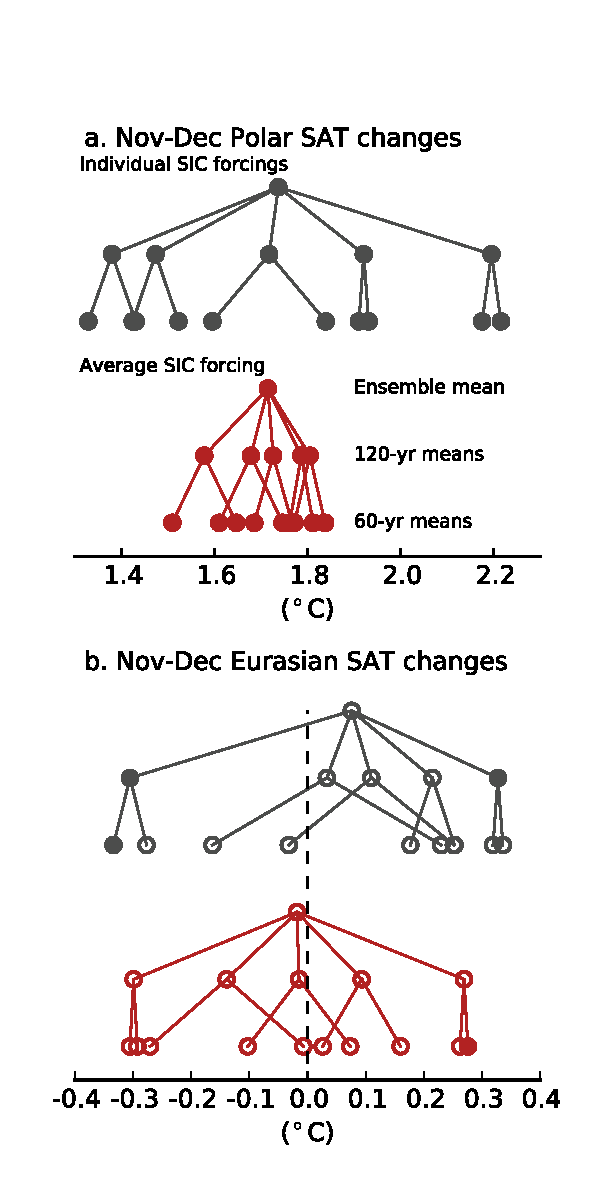
\includegraphics[width=19pc,angle=0]{fig2.pdf} \\ 
  \caption{Regional November-December response of SAT to Individual SIC forcings (black) and Average SIC forcing (red) shown as uncertainty cascades of the a.) polar cap anomalies (averaged poleward of 60$^\circ$N) and b.) Eurasian anomalies (averaged within 35$^\circ$N-60$^\circ$N, 40$^\circ$E-120$^\circ$E). Each cascade consists of the ensemble average of five 120-year ensemble members (top level),  individual 120-year ensemble member averages (middle level), and ensemble members sub-sampled into two 60-year segment averages (bottom level). Filled circles indicate significance at the 95\% level using the Student's T test of difference between two means.
}\label{fig:fig2}
\end{figure}

\begin{figure}[t]
  \noindent\includegraphics[width=20pc,angle=0]{wacefigure3.pdf} \\ 
  \caption{November-December averaged Eurasian SAT changes ($^\circ$C) with geopotential heights at 500 hPa in contours (contour interval = 3 m).
}\label{fig:fig3}
\end{figure} % Z500 contours  [-15. -12.  -9.  -6.  -3.   0.   3.   6.   9.  12.  15.]

\begin{figure}[t]
  \noindent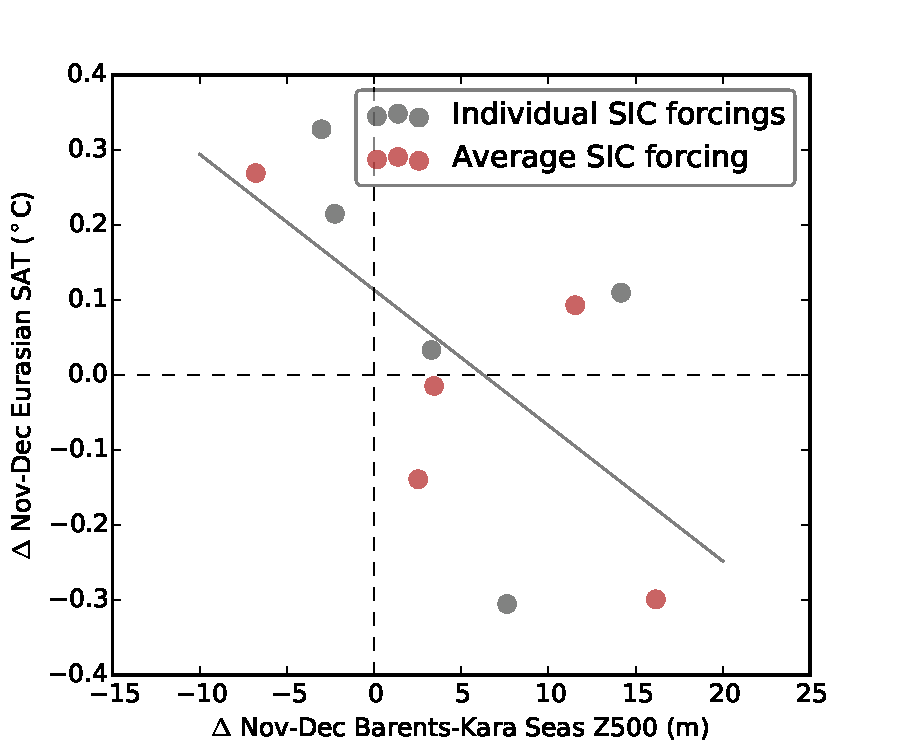
\includegraphics[width=20pc,angle=0]{fig4.pdf} \\ 
  \caption{November-December averaged Eurasian SAT versus geopotential heights at 500 hPa over the Barents-Kara Seas region (65$^\circ$N - 80$^\circ$N, 27$^\circ$E - 96$^\circ$E). $r^2 = 0.39$, $p = 0.05$
}\label{fig:fig4}
\end{figure}

\section{Discussion}

% Discussion?
It is common practice to isolate the impact of Arctic sea ice loss on the midlatitudes by analyzing simulations of 60-100 ensemble members or years (e.g. Screen13, Alexander04, Liu12). We have told a cautionary tale in which significance even at the 120-year level may not be robust in larger ensembles.

We emphasize that these results do not contradict studies that show physical mechanisms consistent with Arctic sea-ice loss causing colder Eurasian SAT in winter. 

While observed Arctic sea-ice loss may well be connected to recent colder Eurasian winters, our results suggest that it is a factor of internal variability --- both in response to sea-ice loss and potentially in the sea ice loss pattern itself --- or due to other factors such as North Atlantic sea surface temperatures (cite Peings14, Sato14). We find that the robust response to human-induced sea-ice loss is a slight warming that is not statistically different from zero $^\circ$C.

%%% End of body of article:

%%%%%%%%%%%%%%%%%%%%%%%%%%%%%%%%
%% Optional Appendix goes here
%
% \appendix resets counters and redefines section heads
% but doesn't print anything.
% After typing  \appendix
%
% \section{Here Is Appendix Title}
% will show
% Appendix A: Here Is Appendix Title
%
%%%%%%%%%%%%%%%%%%%%%%%%%%%%%%%%%%%%%%%%%%%%%%%%%%%%%%%%%%%%%%%%
%
% Optional Glossary or Notation section, goes here
%
%%%%%%%%%%%%%%
% Glossary is only allowed in Reviews of Geophysics
% \section*{Glossary}
% \paragraph{Term}
% Term Definition here
%
%%%%%%%%%%%%%%
% Notation -- End each entry with a period.
% \begin{notation}
% Term & definition.\\
% Second term & second definition.\\
% \end{notation}
%%%%%%%%%%%%%%%%%%%%%%%%%%%%%%%%%%%%%%%%%%%%%%%%%%%%%%%%%%%%%%%%
%
%  ACKNOWLEDGMENTS

\begin{acknowledgments}
(Text here)
\end{acknowledgments}

%% ------------------------------------------------------------------------ %%
%%  REFERENCE LIST AND TEXT CITATIONS
%
% Either type in your references using
% \begin{thebibliography}{}
% \bibitem{}
% Text
% \end{thebibliography}
%
% Or,
%
% If you use BiBTeX for your references, please produce your .bbl
% file and copy the contents into your paper here.
%
% Follow these steps:
% 1. Run LaTeX on your LaTeX file.
%
% 2. Run BiBTeX on your LaTeX file.
%
% 3. Open the new .bbl file containing the reference list and
%   copy all the contents into your LaTeX file here.
%
% 4. Comment out the old \bibliographystyle and \bibliography commands.
%
% 5. Run LaTeX on your new file before submitting.
%
% AGU DOES NOT WANT a .bib or a .bbl file. Please copy in the contents of your .bbl file here.

%\bibliographystyle{plain}
\clearpage
%\bibliographystyle{/Users/kelly/Dropbox/latexbib/ametsoc}
%\bibliography{/Users/kelly/Dropbox/latexbib/allrefs}
\bibliographystyle{ametsoc}
\bibliography{allrefs}


%\begin{thebibliography}{}

%\bibitem[{\textit{Kilby}(2008)}]{jskilby}
%Kilby, J. S. (2008), Invention of the integrated circuit, {\it IEEE
%Trans. Electron Devices,} \textit{23}, 648--650.

%\bibitem[{\textit{Kilby et al.}(2008)}]{jskilbye}
%Kilby, J. S., S. Smith, and R. Jones (2008), Invention of the
%integrated circuit, {\it IEEE Trans. Electron Devices,} \textit{23},
%648--650.

%\end{thebibliography}

%Reference citation examples:

%...as shown by \textit{Kilby} [2008].
%...as shown by {\textit  {Lewin}} [1976], {\textit  {Carson}} [1986], {\textit  {Bartholdy and Billi}} [2002], and {\textit  {Rinaldi}} [2003].
%...has been shown [\textit{Kilby et al.}, 2008].
%...has been shown [{\textit  {Lewin}}, 1976; {\textit  {Carson}}, 1986; {\textit  {Bartholdy and Billi}}, 2002; {\textit  {Rinaldi}}, 2003].


%...as shown by \citet{jskilby}.
%...as shown by \citet{lewin76}, \citet{carson86}, \citet{bartoldy02}, and \citet{rinaldi03}.
%...has been shown \citep{jskilbye}.
%...has been shown \citep{lewin76,carson86,bartoldy02,rinaldi03}.
%
% Please use ONLY \citet and \citep for reference citations. 
% DO NOT use other cite commands (e.g., \cite, \citeyear, \nocite, \citealp, etc.).

%% ------------------------------------------------------------------------ %%
%
%  END ARTICLE
%
%% ------------------------------------------------------------------------ %%

\end{article}

%% Enter Figures and Tables here:

% When submitting articles through the GEMS system:
% COMMENT OUT ANY COMMANDS THAT INCLUDE GRAPHICS.

% Figure captions go below the figure.
% Table titles go above tables; all other caption information 
%  should be placed in footnotes below the table.


% DRAFT figure/table, including eps graphics
%
% \begin{figure}
% \noindent\includegraphics[width=20pc]{samplefigure.eps}
% \caption{Caption text here}
% \end{figure}
% \end{document}
%
% \begin{table}
% \caption{}
% \end{table}
%
% ---------------
% TWO-COLUMN figure/table
%
% \begin{figure*}
% \noindent\includegraphics[width=39pc]{samplefigure.eps}
% \caption{Caption text here}
% \end{figure*}
%
% \begin{table*}
% \caption{Caption text here}
% \end{table*}
%
% ---------------
% EXAMPLE TABLE
%
%\begin{table}
%\caption{Time of the Transition Between Phase 1 and Phase 2\tablenotemark{a}}
%\centering
%\begin{tabular}{l c}
%\hline
% Run  & Time (min)  \\
%\hline
%  $l1$  & 260   \\
%  $l2$  & 300   \\
%  $l3$  & 340   \\
%  $h1$  & 270   \\
%  $h2$  & 250   \\
%  $h3$  & 380   \\
%  $r1$  & 370   \\
%  $r2$  & 390   \\
%\hline
%\end{tabular}
%\tablenotetext{a}{Footnote text here.}
%\end{table}

% See below for how to make landscape/sideways figures or tables.

\end{document}

%%%%%%%%%%%%%%%%%%%%%%%%%%%%%%%%%%%%%%%%%%%%%%%%%%%%%%%%%%%%%%%

More Information and Advice:

%% ------------------------------------------------------------------------ %%
%
%  SECTION HEADS
%
%% ------------------------------------------------------------------------ %%

% Capitalize the first letter of each word (except for
% prepositions, conjunctions, and articles that are
% three or fewer letters).

% AGU follows standard outline style; therefore, there cannot be a section 1 without
% a section 2, or a section 2.3.1 without a section 2.3.2.
% Please make sure your section numbers are balanced.
% ---------------
% Level 1 head
%
% Use the \section{} command to identify level 1 heads;
% type the appropriate head wording between the curly
% brackets, as shown below.
%
%An example:
%\section{Level 1 Head: Introduction}
%
% ---------------
% Level 2 head
%
% Use the \subsection{} command to identify level 2 heads.
%An example:
%\subsection{Level 2 Head}
%
% ---------------
% Level 3 head
%
% Use the \subsubsection{} command to identify level 3 heads
%An example:
%\subsubsection{Level 3 Head}
%
%---------------
% Level 4 head
%
% Use the \subsubsubsection{} command to identify level 3 heads
% An example:
%\subsubsubsection{Level 4 Head} An example.
%
%% ------------------------------------------------------------------------ %%
%
%  IN-TEXT LISTS
%
%% ------------------------------------------------------------------------ %%
%
% Do not use bulleted lists; enumerated lists are okay.
% \begin{enumerate}
% \item
% \item
% \item
% \end{enumerate}
%
%% ------------------------------------------------------------------------ %%
%
%  EQUATIONS
%
%% ------------------------------------------------------------------------ %%

% Single-line equations are centered.
% Equation arrays will appear left-aligned.

Math coded inside display math mode \[ ...\]
 will not be numbered, e.g.,:
 \[ x^2=y^2 + z^2\]

 Math coded inside \begin{equation} and \end{equation} will
 be automatically numbered, e.g.,:
 \begin{equation}
 x^2=y^2 + z^2
 \end{equation}

% IF YOU HAVE MULTI-LINE EQUATIONS, PLEASE
% BREAK THE EQUATIONS INTO TWO OR MORE LINES
% OF SINGLE COLUMN WIDTH (20 pc, 8.3 cm)
% using double backslashes (\\).

% To create multiline equations, use the
% \begin{eqnarray} and \end{eqnarray} environment
% as demonstrated below.
\begin{eqnarray}
  x_{1} & = & (x - x_{0}) \cos \Theta \nonumber \\
        && + (y - y_{0}) \sin \Theta  \nonumber \\
  y_{1} & = & -(x - x_{0}) \sin \Theta \nonumber \\
        && + (y - y_{0}) \cos \Theta.
\end{eqnarray}

%If you don't want an equation number, use the star form:
%\begin{eqnarray*}...\end{eqnarray*}

% Break each line at a sign of operation
% (+, -, etc.) if possible, with the sign of operation
% on the new line.

% Indent second and subsequent lines to align with
% the first character following the equal sign on the
% first line.

% Use an \hspace{} command to insert horizontal space
% into your equation if necessary. Place an appropriate
% unit of measure between the curly braces, e.g.
% \hspace{1in}; you may have to experiment to achieve
% the correct amount of space.


%% ------------------------------------------------------------------------ %%
%
%  EQUATION NUMBERING: COUNTER
%
%% ------------------------------------------------------------------------ %%

% You may change equation numbering by resetting
% the equation counter or by explicitly numbering
% an equation.

% To explicitly number an equation, type \eqnum{}
% (with the desired number between the brackets)
% after the \begin{equation} or \begin{eqnarray}
% command.  The \eqnum{} command will affect only
% the equation it appears with; LaTeX will number
% any equations appearing later in the manuscript
% according to the equation counter.
%

% If you have a multiline equation that needs only
% one equation number, use a \nonumber command in
% front of the double backslashes (\\) as shown in
% the multiline equation above.

%% ------------------------------------------------------------------------ %%
%
%  LANDSCAPE/SIDEWAYS FIGURE AND TABLE EXAMPLES
%
%% ------------------------------------------------------------------------ %%
%
% For figures, add \usepackage{lscape} to the file and the landscape.sty style file
% to the paper folder.
%
% \begin{figure*}[p]
% \begin{landscapefigure*}
% Illustration here.
% \caption{caption here}
% \end{landscapefigure*}
% \end{figure*}
%
% For tables, add \usepackage{rotating} to the paper and add the rotating.sty file to the folder.
%
% AGU prefers the use of {sidewaystable} over {landscapetable} as it causes fewer problems.
%
% \begin{sidewaystable}
% \caption{}
% \begin{tabular}
% Table layout here.
% \end{tabular}
% \end{sidewaystable}
%
%

